% !TEX root = main-dami.tex

\section{Overview}
\label{ch5-sec:overview}
The crime data collected in Chicago has detailed information about time, location (i.e., latitude and longitude), and types of crime. In our problem, the term \emph{crime count} refers to number of crime incidents in a region (i.e., community area) in a year. The \emph{community area} is used as our geographical unit of study, since it is well-defined,  historically recognized and stable over time~\cite{SrGc09}. In total, there are 77 community areas in Chicago.  \emph{Crime rate} is the crime count normalized by the population in a region. We use vector $\y = [y_1, y_2, \ldots, y_n]^T$ to denote the crime rates in regions. The crime rate inference problem is to estimate the crime rate in one region using the crime rate of other regions in the same year by considering the features of regions and correlations among regions. 


The crime data of Chicago are obtained from the City of Chicago data portal~\cite{crime-data}. Chicago is one of few cities with detailed crime data that are made public online. The crime dataset contains the incident date, location (street name and GPS coordinates), and primary type from year 2001 to 2015. In total there are \num{5856414} recorded crime incidents over 15 years, or on average \num{390417} crimes incidents per year. We visualize the crime rate in Figure~\ref{fig:crime-ca}, from which we can see that the downtown area has the highest crime rate.

\begin{figure}[t]
\centering
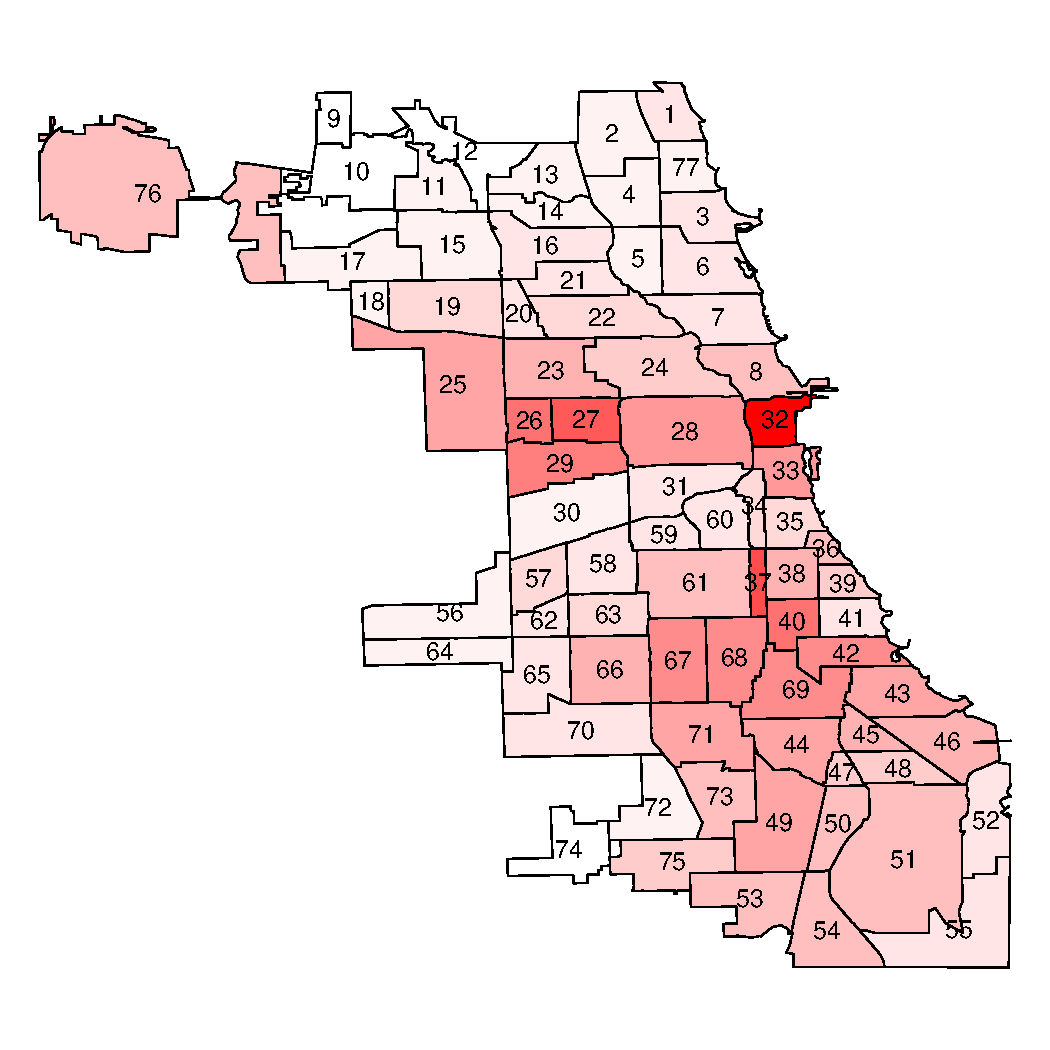
\includegraphics[width=0.6\linewidth]{fig/crime-ca.pdf}
\caption{Crime rate of Chicago by community areas. The community area \#32 is Chicago downtown, which has the highest crime rate.}
\label{fig:crime-ca}
\end{figure}


In this chapter we use the crime rate inference problem as an example, and apply a non-stationary spatial model. More specifically, we estimate the crime rate of some regions given the information of all the other regions. Without loss of generality, we assume there is one community area $t$ with crime rate $y_t$ missing, and we use the crime rate of all the other regions $\{y_i \} \backslash y_t$ to infer this missing value. Our problem is mathematically formalized as follows
\begin{equation}
\hat{y_t} = f( \{y_i\} \backslash y_t, X),
\end{equation}
where  $X$ refers to observed extra information of  all those community areas.




\smallskip
We consider two types of features $X$ for inference:
\begin{itemize}[leftmargin=*]
\item {\bf Nodal features:} Nodal features describe the characteristics of the focal region. Such features include demographic information and Point-of-Interest (POI) distribution. Demographics are frequently used in literature, but POI is a newer type of big data, which we find significantly improve the crime inference accuracy.
\item {\bf Edge features:} (1) Geographical influence. Geographical influence considers the crime rate of the nearby locations.  This feature has been extensively used in literature as well. To estimate the focal region, the crime rate of nearby regions are weighted according to spatial distances. (2) Hyperlink by taxi flow. Locations are connected through the frequent trips made by humans, which can be considered as the hyperlinks in space. This type of feature has not been previously studied in the criminology literature. We propose to use taxi trips to construct the social flow. Our hypothesis is that two regions that are more strongly connected through social flow will influence each other's crime rate.
\end{itemize}

We construct these two types of features using a similar approach in Section~\ref{ch2-sec:feature}.


